
Voici l'enregistrement de la vitesse à chaque instant d'une monoplace lors du Grand Prix de Monaco.

\begin{center}
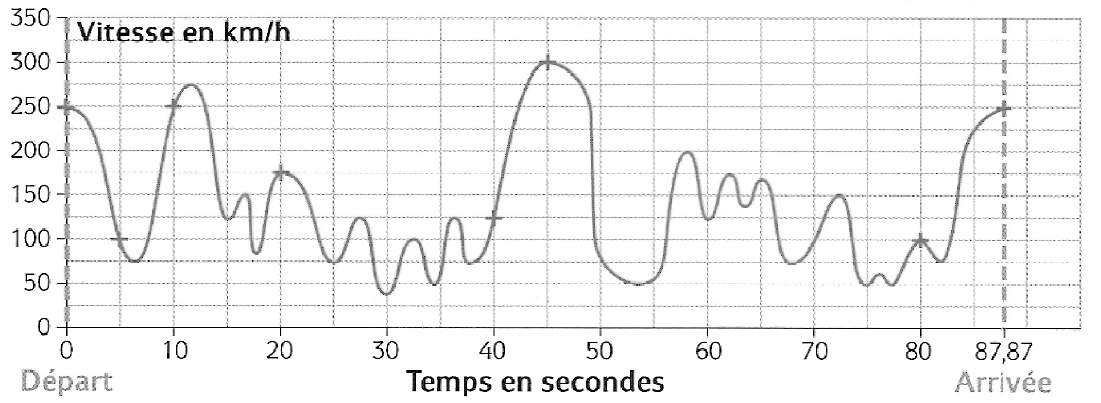
\includegraphics[scale=0.6]{NF-47.png} 
\end{center}

\begin{enumerate}
\item Lors de son passage sur la ligne de départ, la voiture était-elle arrêtée ou lancée ?
\item Recopier et compléter :"Ce graphique représente les variations de la $\dots \ldots$ de la voiture en fonction du $\ldots \ldots$
\item Lire la vitesse de la voiture au bout de $ 5s \quad 20s \quad 40s \quad 80s $.
\item Lire les instants aux la voiture à roulé à 300 km/h, 250 km/h et 25 km/h.
\end{enumerate}